\documentclass[journal]{IEEEtran}
\usepackage{cite}
\usepackage{amsmath,amssymb}
\usepackage{graphicx}
\usepackage{booktabs}
\usepackage[table]{xcolor}
\usepackage{siunitx}
\usepackage{tikz}
\usetikzlibrary{arrows.meta,calc,positioning,shapes.geometric}
\usepackage{hyperref}
\hypersetup{hidelinks}
\sisetup{round-mode=places,round-precision=4}
\hbadness=10000
\hfuzz=20pt

\newcommand{\tablestyle}[2]{\setlength{\tabcolsep}{#1}\renewcommand{\arraystretch}{#2}}
\newcommand{\tablefontsize}{\fontsize{7.2pt}{8.4pt}\selectfont}
\newcommand\headspace{\hspace{.2em}}

\title{Conditional Drifting Models for Learned Channel Simulation}

\author{
\IEEEauthorblockN{Rick Fritschek and Rafael F. Schaefer}
\IEEEauthorblockA{TU Dresden, Germany}
}

\begin{document}
\maketitle

\begin{abstract}
Accurate stochastic channel simulation is central to data-driven communication system design, especially when measured channels are costly to acquire repeatedly or when differentiable learned surrogates are needed inside end-to-end optimization loops.
Recent work has shown that conditional diffusion models are strong channel generators, but their inference cost scales with the number of reverse denoising steps.
This paper studies conditional drifting models as a low-latency alternative and evaluates them against conditional DDPM, conditional DDIM, and conditional WGAN baselines.
We evaluate two drifting variants: residual drifting, which models \(e = y - x\), and conditional (direct-output) drifting, which models \(p(y\mid x)\) directly.
The benchmark covers AWGN, Rayleigh fading, SSPA nonlinearity, and a simplified optical-fiber proxy channel.
Both drifting variants adapt the drifting-model idea to conditional channel generation by using attraction--repulsion drift fields in their respective output spaces.
We show that diffusion baselines provide the strongest SWD overall, while both drifting variants remain competitive. Moreover, a timing study shows that one-shot drifting retains microsecond-level inference while diffusion samplers remain in the millisecond regime.
These results position drifting as a promising fast alternative to iterative diffusion-based channel generators.
\end{abstract}

\begin{IEEEkeywords}
learned channel models, conditional generative modeling, diffusion models, drifting models, sliced Wasserstein distance, inference latency
\end{IEEEkeywords}

\section{Introduction}
Accurate channel models are a basic requirement for modern communication-system design.
They are especially important in neural and end-to-end learned systems, where the channel appears repeatedly inside training loops, decoder adaptation procedures, and differentiable autoencoder pipelines.
When a clean analytical channel model is unavailable, too restrictive, or poorly matched to measured data, generative channel surrogates become attractive because they can learn the full conditional distribution directly from samples.

This problem is not only about distributional accuracy.
In many learning pipelines, the channel model is evaluated millions of times.
As a result, sample quality, conditioning accuracy, computational cost, and differentiability all matter simultaneously.
The question is therefore not merely whether a generative model can match the channel distribution, but whether it can do so at a cost compatible with large-scale training and deployment workflows.

Recent work on diffusion-based channel modeling has shown that conditional diffusion models can generate high-quality channel samples across standard benchmarks such as AWGN, Rayleigh, and nonlinear amplifier channels \cite{paper2309}.
Follow-up work has further studied robustness and speed-quality tradeoffs for diffusion-based channel generation \cite{kimicc2024}, extended diffusion-based channel synthesis to high-dimensional user-specific channels \cite{lee2024highdimchannels}, and proposed diffusion-driven digital-twin style generation of statistical channel state information from sensing and location information \cite{gong2025dtoc}.
More broadly, diffusion methods have also begun to influence adjacent wireless tasks such as high-dimensional channel estimation \cite{zhou2025channelestimation}, low-complexity MIMO channel estimation \cite{fesl2024mimoestimation,chen2025mimovi}, joint channel estimation and data detection \cite{zilberstein2024joint}, and fast time-varying MIMO-OFDM estimation \cite{liu2025mimoofdm}.
That line of work is compelling because diffusion models are flexible, robust, and often more stable than earlier adversarial approaches.
However, this improvement comes with a practical systems cost: inference requires an iterative reverse denoising procedure, and the latency scales with the number of diffusion steps.
This tradeoff is manageable when the channel generator is called occasionally, but it becomes more problematic when it is embedded in inner loops of iterative training or repeated Monte Carlo evaluation. This latency bottleneck has motivated several acceleration strategies for diffusion, including skipped or reduced-step sampling as in DDIM, as well as one-step or few-step alternatives such as consistency models and distillation-based approaches that compress multi-step samplers into substantially shorter generation paths \cite{ddim,song2023consistency,yin2024onestep}.
This motivates the study of one-shot conditional generators for learned channel simulation.
Among recently proposed generative paradigms, drifting models \cite{drifting} are particularly interesting because they aim to learn the transport from a simple latent source to the target data distribution directly in the network parameters, rather than unfold that transport as a multi-step sampling trajectory at inference time.
Intuitively, diffusion spends computation at test time by progressively transforming noise into data through a reverse-time chain.
Drifting instead spends computation during training: generated samples are repeatedly nudged toward the data manifold by a drift field, and the neural generator is updated so that future samples move closer to the desired distribution in a single forward pass.
Once trained, sampling is therefore naturally one-shot.
This perspective is also consistent with recent geometric analyses of generative dynamics that relate diffusion-like behavior to autonomous vector-field structure and marginalized noise geometry \cite{geometryofnoise}.

That distinction makes drifting conceptually appealing for channel modeling.
In a communication setting, the generator must be conditional on the transmitted symbol \(x\), and it must capture not just a marginal sample cloud, but the conditional law \(p(y \mid x)\).
Because drifting was introduced very recently, no widely adopted communication-channel baseline has yet emerged.
This motivates reporting not only benchmark outcomes, but also the concrete conditional adaptation needed to integrate drifting into an existing channel-learning pipeline.

The emphasis of this study is on generator-level distributional accuracy and computational tradeoffs rather than on downstream symbol-error-rate curves.

The main contributions are summarized as follows.
\begin{itemize}
\item We formulate conditional drifting generators for channel simulation in both residual form,
  using \(e = y - x\), and direct-output form, modeling \(p(y \mid x)\) directly.
\item We provide a practical drifting objective based on attraction and repulsion in the chosen
  target space, which is straightforward to integrate into an existing PyTorch channel-learning
  pipeline.
\item We compare the resulting drifting variants against conditional DDPM, conditional DDIM, and
  conditional WGAN models on AWGN, Rayleigh, SSPA, and optical-fiber proxy channels.
\item We quantify the accuracy--latency tradeoff and show that one-shot drifting provides large inference-time savings while remaining competitive in distributional accuracy.
\end{itemize}
Code will be released upon publication\footnote{Code repository: \url{https://github.com/Fritschek}.}.

\section{Problem Formulation and Drifting Background}
\subsection{What drifting changes conceptually}
Because drifting is very recent and remains less familiar than diffusion, we briefly summarize its generative viewpoint.
Following \cite{drifting}, let \(f_\theta\) map a latent variable \(z \sim p_z\) to a sample \(u = f_\theta(z)\), and let
\begin{equation}
q_\theta = (f_\theta)_\# p_z
\end{equation}
denote the pushforward distribution induced by the generator.
The training objective is no longer expressed as a likelihood surrogate or as a denoising score-matching loss.
Instead, the paper introduces a \emph{drifting field} that tells us how samples drawn from the current model distribution should move so that the model distribution approaches the target distribution \(p\).

At a high level, the desired property is an equilibrium condition:
if the model already matches the target distribution, then the drift should vanish.
Using \(V_{p,q}(u)\) to denote the field evaluated at a sample \(u\) under target distribution \(p\) and model distribution \(q\), the fixed-point intuition can be summarized as
\begin{equation}
q = p
\quad \Longrightarrow \quad
V_{p,q}(u) = 0,
\end{equation}
which is the sense in which matched distributions form an equilibrium of the training dynamics \cite{drifting}.

This makes the training logic very different from diffusion.
In diffusion, one learns a denoiser and then performs iterative refinement at inference time.
In drifting, one instead constructs improved targets during training by moving current samples along the field \(V_{p,q}\), and then regresses the generator onto those improved targets.
As a result, the iterative correction happens during optimization rather than at test time.

The one-step view can be written as follows.
Starting from a generated sample \(u = f_\theta(z)\), define a drifted target
\begin{equation}
\tilde{u}
=
\mathrm{stopgrad}\!\left(
u + \eta V_{p,q_\theta}(u)
\right),
\end{equation}
and optimize the generator by
\begin{equation}
\mathcal{L}_{\text{drift}}
=
\mathbb{E}_{z \sim p_z}
\left[
\left\|
f_\theta(z) - \tilde{u}
\right\|_2^2
\right].
\end{equation}
The stop-gradient is essential here: it makes the drifted sample behave like a fixed target for the current optimization step.
Repeated training steps therefore evolve the pushforward \(q_\theta\) toward the target distribution.
This is also the cleanest way to see why drifting is naturally one-shot at inference:
once the generator has learned to emit samples near equilibrium, sampling only requires drawing \(z\) and evaluating \(f_\theta(z)\), with no reverse-time chain.

Fig.~\ref{fig:toy} gives an actual toy particle simulation in the spirit of the particle-based demonstrations used in \cite{drifting}.
For two fixed channel inputs, we initialize mismatched conditional residual particle clouds and then evolve them under the same attraction--repulsion drift rule used in our channel benchmark.
The figure therefore illustrates real drift dynamics rather than a hand-drawn schematic, while still serving only as a toy analogue of the full learned generator.
To show that the same idea can train an explicit parameterized generator, Fig.~\ref{fig:toymlp} uses a tiny conditional MLP trained with the drifting objective on the same toy target.
%For contrast, Fig.~\ref{fig:toydiff} shows an oracle conditional diffusion-style reverse trajectory on the same target, making the difference in sampling path length visually explicit.

\subsection{Conditional channel simulation}
We now specialize the generic drifting view to learned conditional channel simulation.
Let \(x \in \mathbb{R}^n\) denote the transmitted channel input and \(y \in \mathbb{R}^n\) the channel output.
The objective is to learn a conditional generator that reproduces the channel law given \(x\).
In this setting, conditioning enters through the transmitted symbol, while stochasticity is carried by a latent variable \(z \sim \mathcal{N}(0, I)\).

Two target parameterizations are useful in the experiments.
The first is the direct channel-output formulation, in which the generator approximates \(p(y \mid x)\) and predicts \(\hat{y} = g_\theta(x, z)\).
The second is the residual formulation, in which
\begin{equation}
e = y - x
\end{equation}
is modeled instead, so that the generator approximates \(p(e \mid x)\) and the channel output is reconstructed as
\begin{equation}
\hat{y} = x + \hat{e}.
\end{equation}
The direct formulation corresponds to learning the channel law itself, whereas the residual formulation injects the inductive bias that the channel output can be understood as the transmitted symbol plus a structured perturbation.
As discussed later in the experiments, the direct formulation is a natural continuation to direct-output diffusion and WGAN baselines, while the residual formulation is easier to optimize but can also fall short in non-linear channels.

\begin{table}[t]
\caption{\textbf{Two target parameterizations for conditional drifting.}}
\label{tab:drifting_modes}
\centering
\tablestyle{5pt}{1.03}
\tablefontsize
\begin{tabular}{@{}p{1.0cm}p{1.50cm}p{1.60cm}p{2.00cm}@{}}
\toprule
Mode & Output of \(g_\theta\) & Target object & Short interpretation \\
\midrule
Direct & \(\hat y\) & Learn \(p(y \mid x)\) & Learns the channel law directly\\
Residual & \(\hat e\), then \(\hat y=x+\hat e\) & Learn \(p(e \mid x)\) with \(e=y-x\) & Learns the channel perturbation\\
\bottomrule
\end{tabular}
\end{table}

\subsection{Conditional drifting model}
  We use a practical conditional adaptation inspired by \cite{drifting}.
  To avoid confusion with the communication input symbol \(x\), we use \(u\) above for the generic
  sample variable in the abstract formulation and reserve \(x\) below for the transmitted symbol.
  In our implementation, drifting can be applied either in direct-output space or in residual space.
  In direct mode, the generator predicts \(\hat y = g_\theta(x,z)\); in residual mode, it predicts
  \(\hat e = g_\theta(x,z)\) with reconstruction \(\hat y = x + \hat e\), where
  \begin{equation}
  z \sim \mathcal{N}(0, I).
  \end{equation}
  In both cases, \(g_\theta\) is implemented as a two-hidden-layer multilayer perceptron with hidden
  width \(128\), latent dimension \(16\), and SiLU activations:
\begin{equation}
[x, z]
\rightarrow
\mathrm{Linear}
\rightarrow
\mathrm{SiLU}
\rightarrow
\mathrm{Linear}
\rightarrow
\mathrm{SiLU}
\rightarrow
\mathrm{Linear}.
\end{equation}
The training target is formed from an attraction--repulsion drift field in the chosen target space. This is a concrete channel-specific instantiation of the generic field \(V_{p,q}\).
Given generated samples \(G = \{g_i\}\) and positive samples \(P = \{p_j\}\), we compute
\begin{equation}
V(g_i)
=
\left(
\sum_j w^{(P)}_{ij} p_j - g_i
\right)
-
\lambda
\left(
\sum_k w^{(G)}_{ik} g_k - g_i
\right),
\end{equation}
where \(w^{(P)}\) and \(w^{(G)}\) are row-normalized RBF kernel weights.
The first term attracts each generated sample toward a local barycenter of true samples in the chosen target space, and the second term repels it from nearby generated samples to reduce collapse.
This yields a detached target
\begin{equation}
\tilde{g}_i
=
\mathrm{stopgrad}\!\left(g_i + \eta V(g_i)\right),
\end{equation}
and the generator is optimized by
\begin{equation}
\mathcal{L}_{\text{drift}}
=
\frac{1}{N}
\sum_i
\left\|
g_i - \tilde{g}_i
\right\|_2^2.
\end{equation}
In other words, the generic update \(u \mapsto u + \eta V_{p,q}(u)\) from the drifting formulation is realized here with a kernel-based drift field estimated directly from minibatches of true and generated samples in the selected target space.

In the simulations, the drift scale is \(\eta=1.0\), the repulsive weight is \(\lambda=1.0\), the minimum kernel bandwidth is \(0.2\), and the maximum drift norm is \(2.0\).
These settings were chosen because they produced stable residual distributions and materially improved the early AWGN drifting baselines.

The major operational advantage is straightforward:
once training is complete, sampling requires only a single evaluation of \(g_\theta(x,z)\).
In residual mode, this produces a channel residual sample \(\hat e\) followed by reconstruction \(\hat y=x+\hat e\). In direct mode, it produces \(\hat y\) directly.
There is no reverse chain, no ODE solver, and no per-sample iterative schedule at inference.

%\begin{figure*}[t]
%\centering
%\tikzset{
    title/.style={font=\bfseries\large},
    note/.style={align=center, font=\small, text depth=0pt},
    flow/.style={->, thick, draw=black!70},
    boxbluebase/.style={draw=blue!60!black, thick, rounded corners=2mm, fill=blue!10, align=center},
    boxvioletbase/.style={draw=violet!70!black, thick, rounded corners=2mm, fill=violet!12, align=center},
    boxgreenbase/.style={draw=green!50!black, thick, rounded corners=2mm, fill=green!10, align=center},
    boxredbase/.style={draw=red!60!black, thick, rounded corners=2mm, fill=red!10, align=center}
}
\begin{tikzpicture}[
    >=Latex,
    font=\small,
    boxblue/.style={boxbluebase},
    boxviolet/.style={boxvioletbase},
    boxred/.style={boxredbase},
    boxgreen/.style={boxgreenbase},
    attr/.style={->, thick, draw=green!50!black},
    repel/.style={<->, semithick, draw=orange!85!black},
    truedot/.style={circle, draw=blue!70!black, fill=blue!35, inner sep=1.8pt},
    gendot/.style={circle, draw=orange!80!black, fill=orange!50, inner sep=1.8pt},
    targetdot/.style={circle, draw=green!60!black, fill=green!35, inner sep=1.8pt}
]
\fill[white] (-7.4,-4.2) rectangle (3.6,4.3);

\def\cloudxshift{0cm}
\def\cloudyshift{0cm}
\begin{scope}[shift={(\cloudxshift,\cloudyshift)}]
\node[title] at (-1.9,3.75) {Training step for fixed channel input $x$};

% Left panel: inputs and generator
\node[boxblue, minimum width=1.45cm, minimum height=0.72cm] (condx) at (-6.5,1.2) {condition\\$x$};
\node[boxviolet, minimum width=2.10cm, minimum height=0.92cm] (latent) at (-6.5,2.2) {latent draw\\$z \sim \mathcal{N}(0,I)$};
\node[boxviolet, minimum width=2.30cm, minimum height=0.82cm] (gen) at (-3.8,2.2) {generator\\$g_\theta(x,z)$};
\draw[flow, blue!70!black] (condx.east) -- (gen.west);
\draw[flow, violet!80!black] (latent.east) -- (gen.west);

% True channel
\node[boxred, minimum width=1.55cm, minimum height=0.72cm] (truech) at (-6.5,-0.5) {true channel};
\draw[flow, red!70!black] (condx.south) -- (truech.north);
\node[note, red!70!black, text width=2.3cm] at (-6.1,-1.95) {sample $y$, then form\\$e=y-x$};

% Generated residual cloud
\node[note, orange!80!black] at (-0.5,2.25) {\textbf{generated residuals $\hat e_i$}};
\node[gendot] (g1) at (-2.55,1.35) {};
\node[gendot] (g2) at (-2.1,1.7) {};
\node[gendot] (g3) at (-1.7,1.15) {};
\node[gendot] (g4) at (-1.25,1.55) {};
\node[gendot] (g5) at (-1.9,0.8) {};
\draw[flow, violet!80!black] (gen.east) -- (-3.35,1.2);

% True residual cloud
\node[note, blue!70!black] at (1,-0.05) {\textbf{true residuals $e_j$}};
\node[truedot] (p1) at (-0.25,-0.7) {};
\node[truedot] (p2) at (0.2,-0.33) {};
\node[truedot] (p3) at (0.7,-0.88) {};
\node[truedot] (p4) at (1.15,-0.4) {};
\node[truedot] (p5) at (0.45,-1.18) {};
\draw[flow, red!70!black] (truech.east) to[out=10,in=210] (-0.25,-0.7);

% Drifted targets
\node[note, green!50!black] at (2.3,2.25) {\textbf{drifted targets $\tilde e_i$}};
\node[targetdot] (t1) at (-0.85,1.75) {};
\node[targetdot] (t2) at (-0.35,1.98) {};
\node[targetdot] (t3) at (0.15,1.45) {};
\node[targetdot] (t4) at (0.68,1.78) {};
\node[targetdot] (t5) at (0.0,1.15) {};

% Attraction arrows
\draw[attr] (g1) -- (t1);
\draw[attr] (g2) -- (t2);
\draw[attr] (g3) -- (t3);
\draw[attr] (g4) -- (t4);
\draw[attr] (g5) -- (t5);

% Repulsion arrows
\draw[repel] (g1) -- (g2);
\draw[repel] (g2) -- (g4);
\draw[repel] (g3) -- (g5);

\node[note, align=left, anchor=west, text width=2.8cm] at (1.8,1.15) {$V(\hat e_i)$:\\textcolor{green!50!black}{attraction to data}\\+\textcolor{orange!85!black}{repulsion among generated}};

\end{scope}

% Loss box
\node[boxgreen, minimum width=5.2cm, minimum height=1.55cm] (loss) at (-2.25,-2.35) {$\tilde e_i=\mathrm{stopgrad}\!\left(\hat e_i+\eta V(\hat e_i)\right)$\\[2pt]
$\mathcal{L}_{\mathrm{drift}}=\frac{1}{N}\sum_i \|\hat e_i-\tilde e_i\|_2^2$};
\draw[flow] (-0.7,1.45) to[out=-90,in=25] (loss.north east);
\draw[flow] (0.15,1.2) to[out=-90,in=-5] (loss.north east);
\node[note, text width=4.8cm] at (-2.25,-3.2) {Regress $g_\theta$ toward the drifted residual targets.};
\end{tikzpicture}

%\caption{Training-time drifting update for conditional channel residual modeling. For a fixed transmitted symbol \(x\), the generator produces residual samples \(\hat e_i\), which are moved toward the true residual cloud through a drift field that combines attraction to data and repulsion among generated samples. The network is then regressed toward the drifted targets.}
%\label{fig:drifttrain}
%\end{figure*}

%\begin{figure*}[t]
%\centering
%\tikzset{
    title/.style={font=\bfseries\large},
    note/.style={align=center, font=\small, text depth=0pt},
    flow/.style={->, thick, draw=black!70},
    boxbluebase/.style={draw=blue!60!black, thick, rounded corners=2mm, fill=blue!10, align=center},
    boxvioletbase/.style={draw=violet!70!black, thick, rounded corners=2mm, fill=violet!12, align=center},
    boxgreenbase/.style={draw=green!50!black, thick, rounded corners=2mm, fill=green!10, align=center},
    boxredbase/.style={draw=red!60!black, thick, rounded corners=2mm, fill=red!10, align=center}
}
\begin{tikzpicture}[
    >=Latex,
    font=\small,
    boxblue/.style={boxbluebase},
    boxviolet/.style={boxvioletbase},
    boxgreen/.style={boxgreenbase}
]
\fill[white] (-0.5,-2.3) rectangle (8.7,3.1);
\node[title] at (4.0,2.5) {Residual-mode one-shot inference};
\coordinate (inferstart) at (0.2,1.1);
\node[boxblue, minimum width=1.45cm, minimum height=0.95cm, anchor=west] (cond2) at (inferstart) {$x$};
\node[boxviolet, minimum width=1.55cm, minimum height=1.05cm, right=0.28cm of cond2.east, anchor=west] (latent2) {$z$};
\node[boxviolet, minimum width=2.2cm, minimum height=1.05cm, right=0.32cm of latent2.east, anchor=west] (gen2) {$g_\theta(x,z)$};
\node[boxgreen, minimum width=1.7cm, minimum height=1.0cm, right=0.32cm of gen2.east, anchor=west] (ehat) {$\hat e$};
\node[boxgreen, minimum width=2.15cm, minimum height=1.0cm, right=0.32cm of ehat.east, anchor=west] (yhat) {$\hat y=x+\hat e$};
\draw[flow, blue!70!black] (cond2.east) -- (gen2.west);
\draw[flow, violet!80!black] (latent2.east) -- (gen2.west);
\draw[flow, green!50!black] (gen2.east) -- (ehat.west);
\draw[flow, green!50!black] (ehat.east) -- (yhat.west);
\node[note, text width=5.8cm] at (4.1,-0.35) {After training: draw \(z\), evaluate \(g_\theta(x,z)\) once, and reconstruct the channel output as \(\hat y=x+\hat e\).};
\node[note, text width=3.0cm, red!70!black] at (7.35,-1.45) {Constant-depth,\\one-shot sampling.};
\end{tikzpicture}
%\caption{Inference-time schematic for residual-mode conditional drifting. Once the generator has been trained, sampling requires only a single forward pass of \(g_\theta(x,z)\), followed by residual-to-output reconstruction. In the direct-output parameterization, the same one-shot generator would produce \(\hat y\) directly instead of \(\hat e\).}
%\label{fig:schematic}
%\end{figure*}

\begin{figure*}[t]
\centering
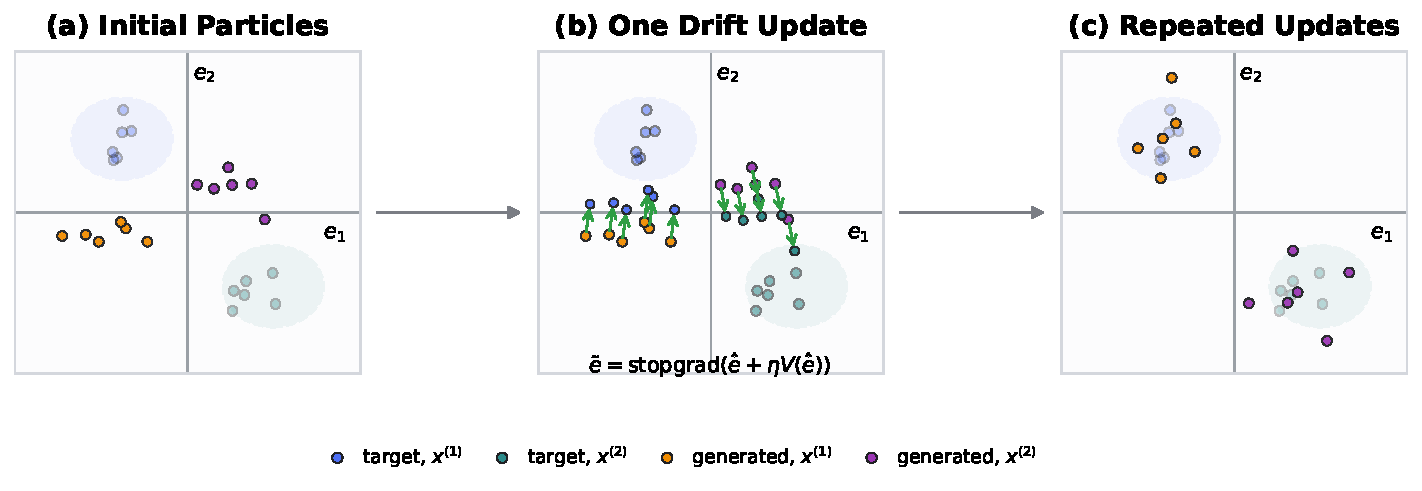
\includegraphics[width=0.7\textwidth]{figures/drifting_conditional_toy_figure_mpl.pdf}
\caption{Toy conditional particle simulation in residual space. Two different channel inputs induce two different target residual distributions. Starting from mismatched generated particle clouds, the middle panel applies one attraction--repulsion drift update of the form \(\tilde e=\mathrm{stopgrad}(\hat e+\eta V(\hat e))\), and the last panel shows the particle clouds after repeated updates. This figure is an actual toy simulation of the drift field, not a hand-drawn schematic.}
\label{fig:toy}
\end{figure*}

\begin{figure*}[t]
\centering
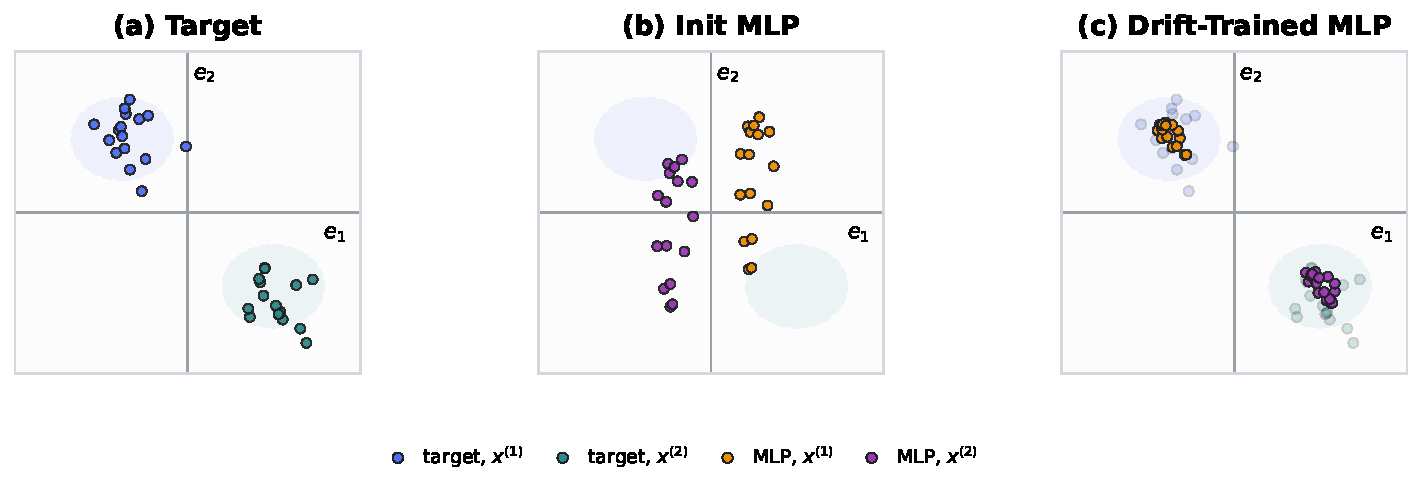
\includegraphics[width=0.7\textwidth]{figures/drifting_tiny_mlp_demo_mpl.pdf}
\caption{Toy conditional MLP trained with the drifting objective. The left panel shows target conditional residual samples. The middle panel shows samples from a randomly initialized tiny conditional MLP \(g_\theta(x,z)\). The right panel shows the same MLP after training with the drift objective, where the generated samples move close to the correct condition-dependent residual clouds.}
\label{fig:toymlp}
\end{figure*}

%\begin{figure*}[t]
%\centering
%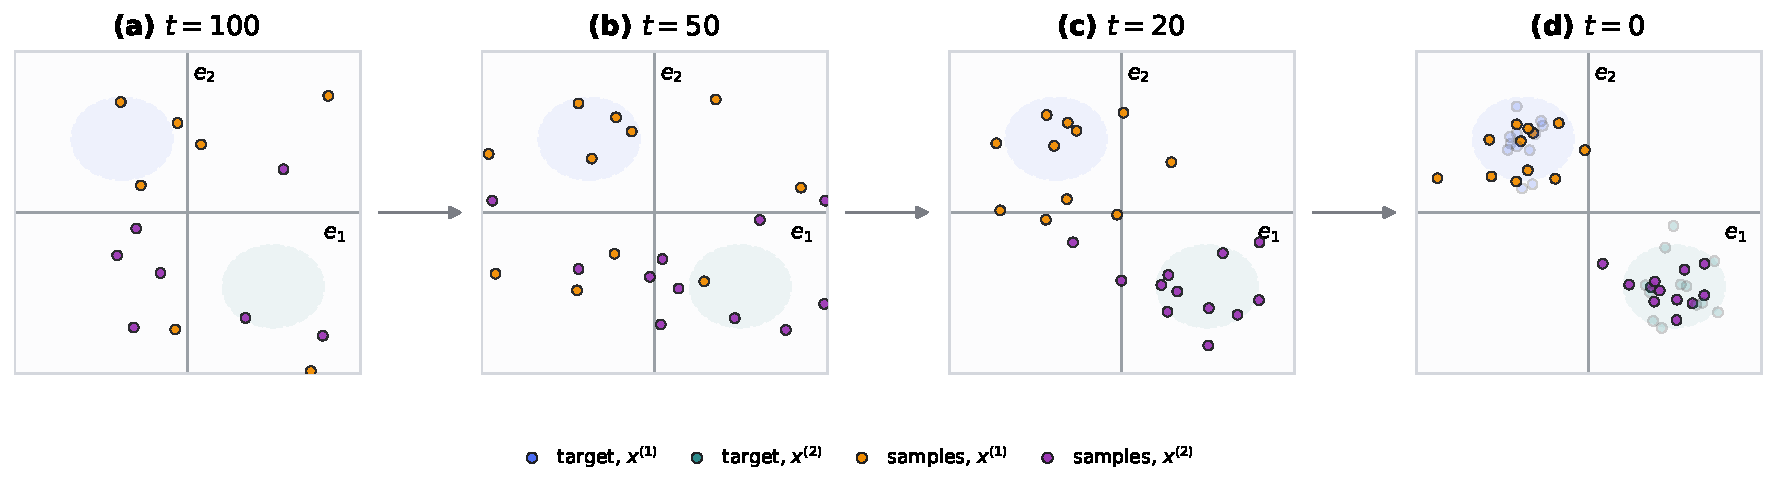
\includegraphics[width=0.7\textwidth]{figures/toy_diffusion_oracle_demo_mpl.pdf}
%\caption{Oracle toy conditional diffusion trajectory on the same Gaussian conditional target. The panels show reverse-time snapshots from a 100-step diffusion process at \(t=100\), \(t=50\), \(t=20\), and \(t=0\). Starting from condition-independent noise, the reverse denoising trajectory progressively separates the conditions and contracts toward their target residual distributions. This figure is included to contrast the explicit multi-step reverse path of diffusion with the one-shot sampling path of drifting.}
%\label{fig:toydiff}
%\end{figure*}

\section{Experimental Setup}
\subsection{Channel models}
We simulate four channel families. All channels are implemented on real-valued vectors.
For AWGN and Rayleigh, we use real-valued channel inputs and output vectors of length \(7\).
For SSPA and OptFib, the real-valued signal is interpreted in paired I/Q coordinates, with dimensions \(8\) and \(2\), respectively.
Noise is independent across real components unless the channel induces coupling.

\textbf{AWGN:}
\begin{equation}
y = x + n,
\qquad
n \sim \mathcal{N}(0,\sigma^2 I).
\end{equation}
This is the standard additive white Gaussian noise reference channel and serves as the simplest near-identity baseline.
\textbf{Rayleigh:}
the transmitted symbol is multiplied elementwise by a random fading amplitude and then corrupted by additive Gaussian noise:
\begin{equation}
y = h \odot x + n,
\end{equation}
where \(\odot\) denotes elementwise multiplication,
\begin{equation}
h_k = \frac{1}{\sqrt{2}}\sqrt{u_k^2 + v_k^2},
\qquad
u_k,v_k \overset{\text{i.i.d.}}{\sim} \mathcal{N}(0,1),
\end{equation}
and $n \sim \mathcal{N}(0,\sigma^2 I).$

Each real component is therefore scaled by an independent Rayleigh-distributed magnitude before noise is added.
This channel is multiplicative rather than additive and is correspondingly less aligned with a pure residual perturbation view.
As implemented here, Rayleigh is also a real-valued vector channel rather than a paired-I/Q complex channel.

\textbf{SSPA:}
the input is passed through a smooth solid-state power amplifier nonlinearity before additive noise is applied.
In this case, the real-valued representation is interpreted as paired I/Q components.
Let
\begin{equation}
r = \sqrt{x_I^2 + x_Q^2}
\end{equation}
denote the input amplitude.
The nonlinear amplitude law used in the benchmark is
\begin{equation}
a(r)
=
\frac{G}{\left(1+\left(\frac{Gr}{A_0}\right)^{2p}\right)^{1/(2p)}},
\end{equation}
with default parameters \(p=3\), \(A_0=1.5\), and \(G=5.0\).
The noiseless amplifier output is $\tilde{x} = a(r)\,x,$
and the observed channel output is
\begin{equation}
y = \tilde{x} + n,
\qquad
n \sim \mathcal{N}\!\left(0,\frac{\sigma^2}{2}I\right).
\end{equation}
This channel introduces amplitude-dependent nonlinear distortion while preserving the input direction in the I/Q plane.

\textbf{OptFib:}
We include a simplified memoryless optical-fiber proxy channel following \cite{li2018e2efiber} for the choice of parameters.
As in SSPA, the real-valued state is interpreted as an I/Q pair.
Let the state after propagation step \(k\) be \(x^{(k)} = [x_I^{(k)},x_Q^{(k)}]^\top\).
At each step, the instantaneous nonlinear phase is
\begin{equation}
\phi^{(k)}
=
\gamma
\left(\left(x_I^{(k)}\right)^2 + \left(x_Q^{(k)}\right)^2\right)\frac{L}{K_{\text{step}}}.
\end{equation}
The deterministic Kerr-style rotation is
\begin{equation}
\begin{aligned}
\tilde{x}_I^{(k+1)} &= x_I^{(k)}\cos\phi^{(k)} - x_Q^{(k)}\sin\phi^{(k)}, \\
\tilde{x}_Q^{(k+1)} &= x_I^{(k)}\sin\phi^{(k)} + x_Q^{(k)}\cos\phi^{(k)},
\end{aligned}
\end{equation}
followed by additive Gaussian perturbations at every step:
\begin{equation}
\begin{aligned}
x_I^{(k+1)} &= \tilde{x}_I^{(k+1)} + \sigma_n \xi_I^{(k)}, \\
x_Q^{(k+1)} &= \tilde{x}_Q^{(k+1)} + \sigma_n \xi_Q^{(k)},
\end{aligned}
\qquad
\xi_I^{(k)},\xi_Q^{(k)} \overset{\text{i.i.d.}}{\sim} \mathcal{N}(0,1).
\end{equation}
When that optical-channel parameterization is used,
\begin{equation}
\sigma_n
=
\sqrt{\frac{10^{(P_n-30)/10}}{2K_{\text{step}}}},
\end{equation}
with \(P_n\) measured in dBm.



\subsection{Training protocol}
This benchmark protocol closely follows the setup in \cite{kimicc2024}.
\paragraph{Channel settings.}
For AWGN and Rayleigh, the setting is \(n=7\), while for SSPA it is \(n=8\). The corresponding \((E_b/N_0, R)\) pairs are \((5\,\mathrm{dB}, 4/7)\) for AWGN, \((12\,\mathrm{dB}, 4/7)\) for Rayleigh, and \((8\,\mathrm{dB}, 6/8)\) for SSPA, yielding noise standard deviations \(0.5260\), \(0.2350\), and \(0.3251\), respectively. For OptFib, the channel parameters are \(L=5000\), \(\gamma=1.27\), \(K_{\text{step}}=50\), and \(P_n=-21.3\) dBm.

\paragraph{Data and optimization settings.}
For AWGN and Rayleigh, we use training dataset size \(10^7\), batch size \(5000\), and \(30\) epochs for drifting, diffusion, and WGAN. For SSPA, we use training dataset size \(10^7\), batch size \(4096\), and \(160\) epochs for all three method families. For these three channels, we evaluate each method on \(10^6\) samples and use \(128\) SWD projections. OptFib is benchmarked separately with training dataset size \(120{,}000\), batch size \(512\), \(60\) training epochs, evaluation size \(100{,}000\), and \(256\) SWD projections.

\paragraph{Model settings.}
Drifting uses a conditional MLP with latent dimension \(16\), hidden width \(128\), two hidden layers, \texttt{SiLU} activations, and Adam with learning rate \(10^{-3}\). The drifting objective uses drift scale \(1.0\), median-heuristic bandwidth selection, minimum bandwidth \(0.2\), maximum drift norm \(2.0\), and repulsive weight \(1.0\). We train both parameterizations: direct drifting with target \(y\) and residual drifting with target \(e=y-x\).

For AWGN, Rayleigh, and SSPA, diffusion models \(p(y\mid x)\) directly with \(v\)-prediction, cosine-ZF variance schedule, \(100\) diffusion steps, and EMA decay \(0.9\). Hidden widths are \(110\) (AWGN), \(128\) (Rayleigh), and \(110\) (SSPA). AWGN and Rayleigh use a two-stage learning-rate schedule (\(10\) epochs at \(10^{-3}\), then \(20\) epochs at \(10^{-4}\)), while SSPA uses a constant \(10^{-4}\) for \(160\) epochs. We report DDPM and DDIM with \(100\), \(50\), \(20\), and \(10\) denoising steps. For OptFib, diffusion uses residual modeling with \(\epsilon\)-prediction, standard cosine schedule, \(100\) steps, hidden width \(128\), learning rate \(10^{-3}\), and EMA decay \(0.995\).

WGAN uses a conditional Wasserstein objective with RMSprop at \(10^{-4}\) for generator and critic, five critic updates per generator update, and weight clipping at \(0.01\). Hidden widths are \(128\) (AWGN) and \(256\) (Rayleigh/SSPA). OptFib uses width \(128\). In the current benchmark implementation, WGAN is reported with residual-space SWD.

To compare distributional accuracy and latency with model capacity, Table~\ref{tab:model-size} reports inference-network parameter counts used in this benchmark.

\begin{table}[t]
\centering
\caption{\textbf{Model parameter counts in the benchmark setup.} Counts refer to inference-time networks. DDPM and DDIM share the same denoiser weights. WGAN rows report generator-side parameters.}
\label{tab:model-size}
\tablestyle{4pt}{1.03}
\tablefontsize
\begin{tabular}{@{}lccc@{}}
\toprule
Model & AWGN & Rayleigh / SSPA & OptFib \\
\midrule
Drifting (direct / residual) & 20{,}487 & 20{,}487 / 20{,}744 & 19{,}202 \\
Diffusion denoiser (DDPM / DDIM) & 59{,}847 & 74{,}247 / 60{,}178 & 72{,}322 \\
WGAN generator & 19{,}335 & 71{,}431 / 72{,}200 & 17{,}410 \\
\bottomrule
\end{tabular}
\end{table}

\paragraph{Seeding and reporting.}
  All benchmark results are reported as mean \(\pm\) standard deviation over ten seeds.
  Each run uses deterministic initialization to reduce run-to-run variance unrelated to model
  stochasticity.
%\paragraph{Seeding and reporting.}
%All runs use deterministic initialization. For AWGN, Rayleigh, and SSPA, the SWD random-projection seed equals the run seed. Final benchmark tables report mean and standard deviation across the ten seeds.

\subsection{Evaluation metric}
We focus on generator-level distributional accuracy and timing rather than full end-to-end communication metrics such as SER or \(E_b/N_0\) curves, to reduce encoder--decoder dependency in the comparison.
The primary metric is sliced Wasserstein distance (SWD), computed in the target space used by each benchmark path.
For direct-output models, we report \(\mathrm{SWD}\!\left(\{\hat{y}_i\}, \{y_i\}\right)\). For residual models, we report \(\mathrm{SWD}\!\left(\{\hat{e}_i\}, \{e_i\}\right)\).
Given true samples \(P=\{v_i\}_{i=1}^N\) and generated samples \(Q=\{\hat v_i\}_{i=1}^N\), SWD is estimated by drawing random unit directions \(\theta_m\), projecting both clouds onto those directions, computing the one-dimensional Wasserstein distance for each projection, and averaging over projections:
\begin{equation*}
\mathrm{SWD}(P,Q)
=
\frac{1}{M}
\sum_{m=1}^M
W_1\!\left(\{\langle \theta_m,v_i\rangle\}_{i=1}^N,\{\langle \theta_m,\hat v_i\rangle\}_{i=1}^N\right).
\end{equation*}
Thus SWD compares the generated and true sample clouds through many one-dimensional views and captures geometric mismatch more faithfully than a purely bin-based marginal comparison. In our experiments, SWD is estimated using \(128\) random one-dimensional projections on AWGN,
  Rayleigh, and SSPA, and \(256\) projections on the separate OptFib benchmark.
SWD is used primarily for comparability with prior diffusion-channel benchmarks \cite{paper2309,kimicc2024}. Compared with histogram-based \(L_1\) distance, it also better captures sample geometry in \(\mathbb{R}^n\).


\section{Benchmark Results}
\subsection{Main SWD benchmark across channels}
Table~\ref{tab:benchmark-all-channels} reports the SWD benchmark across AWGN, Rayleigh, SSPA, and
OptFib. DDIM-100 achieves the lowest SWD on AWGN, Rayleigh, and SSPA, while DDPM is strongest on OptFib. Both drifting variants remain competitive, but their relative strength depends on channel type: residual drifting performs better on AWGN and Rayleigh, whereas direct-output drifting is stronger on SSPA and OptFib. Within this benchmark, residual drifting and WGAN are evaluated in residual space, while direct drifting and diffusion are evaluated in output space. Reduced-step DDIM variants degrade systematically as the number of sampling steps is reduced.
Table~\ref{tab:timing-cuda} summarizes projected CUDA training and inference timing. The main timing result is that one-shot generators operate at microsecond-level inference, whereas diffusion samplers remain in the millisecond regime, yielding a substantial latency gap across all channels.
\begin{table*}[t]
\centering
\caption{\textbf{Ten-seed SWD benchmark across reference channels.} Lower is better. Direct output-space SWD is reported unless the row label explicitly indicates residual-space SWD\@. The residual-space row is included for diagnostic purposes only.}
\label{tab:benchmark-all-channels}
\tablestyle{6.5pt}{1.03}
\tablefontsize
\begin{tabular}{@{}lccc@{}}
\toprule
Method & AWGN & Rayleigh & SSPA \\
\midrule
\rowcolor[gray]{0.9} \multicolumn{4}{l}{\textit{One-shot generators}} \\
\headspace Drifting (dir.) & 0.0100 $\pm$ 0.0007 & 0.0085 $\pm$ 0.0012 & \textbf{0.0060} $\pm$ 0.0008 \\
\headspace Drifting (res., $y$) & 0.0670 $\pm$ 0.0138 & 0.3681 $\pm$ 0.0031 & 0.4812 $\pm$ 0.0022 \\
\headspace Drifting (res., $e$) & \textbf{0.0097} $\pm$ 0.0009 & \textbf{0.0062} $\pm$ 0.0009 & 0.0130 $\pm$ 0.0003 \\
\headspace WGAN & 0.0198 $\pm$ 0.0050 & 0.0171 $\pm$ 0.0050 & 0.0287 $\pm$ 0.0156 \\
\midrule
\rowcolor[gray]{0.9} \multicolumn{4}{l}{\textit{Diffusion samplers}} \\
\headspace DDPM & 0.0070 $\pm$ 0.0004 & 0.0079 $\pm$ 0.0008 & 0.0032 $\pm$ 0.0005 \\
\headspace DDIM-100 & \textbf{0.0042} $\pm$ 0.0006 & \textbf{0.0044} $\pm$ 0.0007 & \textbf{0.0024} $\pm$ 0.0004 \\
\headspace DDIM-50 & 0.0064 $\pm$ 0.0004 & 0.0066 $\pm$ 0.0010 & 0.0030 $\pm$ 0.0005 \\
\headspace DDIM-20 & 0.0143 $\pm$ 0.0003 & 0.0146 $\pm$ 0.0014 & 0.0056 $\pm$ 0.0006 \\
\headspace DDIM-10 & 0.0264 $\pm$ 0.0004 & 0.0271 $\pm$ 0.0013 & 0.0092 $\pm$ 0.0008 \\
\bottomrule
\end{tabular}
\end{table*}


\begin{table*}[t]
\centering
\caption{\textbf{Projected training and inference timing on an NVIDIA RTX 5060 Ti GPU.} Training hours are extrapolated from a 2\% timing run. Inference is reported as time per sample.}
\label{tab:timing-cuda}
\tablestyle{3pt}{1.02}
\tablefontsize
\resizebox{\textwidth}{!}{%
\begin{tabular}{@{}lcccccccccccc@{}}
\toprule
Method & \multicolumn{3}{c}{AWGN} & \multicolumn{3}{c}{Rayleigh} & \multicolumn{3}{c}{SSPA} & \multicolumn{3}{c}{TDL} \\
\cmidrule(lr){2-4} \cmidrule(lr){5-7} \cmidrule(lr){8-10} \cmidrule(lr){11-13}
 & Train [h] & Inf. & Total [h] & Train [h] & Inf. & Total [h] & Train [h] & Inf. & Total [h] & Train [h] & Inf. & Total [h] \\
\midrule
\rowcolor[gray]{0.9} \multicolumn{13}{l}{\textit{One-shot generators}} \\
Drifting (res.) & 1.309 & 0.131 us & 1.310 & 1.300 & 0.123 us & 1.300 & 5.656 & 0.121 us & 5.656 & 0.013 & 0.124 us & 0.013 \\
Drifting (dir.) & 1.299 & 0.114 us & 1.300 & 1.299 & 0.117 us & 1.300 & 5.656 & 0.118 us & 5.656 & 0.007 & 0.116 us & \textbf{0.007} \\
Joint-kernel drift & 1.863 & 0.116 us & 1.864 & 1.864 & 0.116 us & 1.864 & 8.112 & 0.119 us & 8.112 & 0.008 & 0.115 us & 0.008 \\
Joint Sinkhorn & 0.917 & 0.116 us & 0.918 & 0.919 & 0.115 us & 0.920 & 3.956 & 0.117 us & 3.956 & 0.010 & 0.116 us & 0.010 \\
Condition-wise Sinkhorn & 0.048 & 0.115 us & \textbf{0.048} & 0.048 & 0.115 us & \textbf{0.049} & 0.296 & 0.117 us & \textbf{0.297} & 0.009 & 0.115 us & 0.009 \\
WGAN & 0.064 & 0.108 us & 0.064 & 0.085 & 0.108 us & 0.086 & 0.478 & 0.107 us & 0.478 & 0.022 & 0.108 us & 0.022 \\
\midrule
\rowcolor[gray]{0.9} \multicolumn{13}{l}{\textit{Diffusion samplers}} \\
DDPM & 0.020 & 0.046 ms & 0.147 & 0.020 & 0.045 ms & 0.145 & 0.124 & 0.047 ms & 0.253 & 0.005 & 0.045 ms & 0.007 \\
DDIM-100 & 0.020 & 0.039 ms & 0.128 & 0.020 & 0.039 ms & 0.128 & 0.124 & 0.039 ms & 0.231 & 0.005 & 0.039 ms & 0.006 \\
DDIM-50 & 0.020 & 0.019 ms & 0.073 & 0.020 & 0.019 ms & 0.073 & 0.124 & 0.019 ms & 0.177 & 0.005 & 0.019 ms & 0.006 \\
DDIM-20 & 0.020 & 0.008 ms & 0.042 & 0.020 & 0.008 ms & 0.042 & 0.124 & 0.008 ms & 0.145 & 0.005 & 0.008 ms & 0.006 \\
DDIM-10 & 0.020 & 0.004 ms & 0.031 & 0.020 & 0.004 ms & 0.031 & 0.124 & 0.004 ms & 0.135 & 0.005 & 0.004 ms & 0.005 \\
\bottomrule
\end{tabular}
}
\par\vspace{0.25em}
\begin{minipage}{0.96\textwidth}
\footnotesize\raggedright
All rows use the same 2\% extrapolation protocol. In the one-shot block, bold total times mark the lowest projected total for each channel. The W-Flow rows use the same one-shot generator architecture as direct drifting. Their training-time differences come only from the drift-field computation.
\end{minipage}
\end{table*}


\subsection{Direct-space check for residual drifting and WGAN}
To quantify the effect of metric space, we additionally compare residual drifting and WGAN under
both direct \(y\)-space SWD and residual-space SWD in Table~\ref{tab:direct-vs-residual-metric}.
WGAN changes little between the two metrics, whereas residual drifting degrades substantially in direct \(y\)-space, especially on Rayleigh, SSPA, and OptFib. This indicates that residual drifting is well aligned with residual modeling, but that its advantage does not transfer directly to full output-space matching.

\begin{table}[t]
\centering
\caption{\textbf{Direct- and residual-space SWD for residual drifting and WGAN.} Values are ten-seed mean and standard deviation; lower is better.}
\label{tab:direct-vs-residual-metric}
\tablestyle{4pt}{1.03}
\tablefontsize
\begin{tabular}{@{}lcc@{}}
\toprule
Method & Direct SWD & Residual SWD \\
\midrule
\rowcolor[gray]{0.9} \multicolumn{3}{l}{\textit{AWGN}} \\
\headspace Drifting (res.) & 0.0670 $\pm$ 0.0138 & \textbf{0.0103} $\pm$ 0.0010 \\
\headspace WGAN & 0.0198 $\pm$ 0.0050 & \textbf{0.0195} $\pm$ 0.0051 \\
\rowcolor[gray]{0.9} \multicolumn{3}{l}{\textit{Rayleigh}} \\
\headspace Drifting (res.) & 0.3681 $\pm$ 0.0031 & \textbf{0.0063} $\pm$ 0.0011 \\
\headspace WGAN & 0.0171 $\pm$ 0.0050 & \textbf{0.0170} $\pm$ 0.0050 \\
\rowcolor[gray]{0.9} \multicolumn{3}{l}{\textit{SSPA}} \\
\headspace Drifting (res.) & 0.4812 $\pm$ 0.0022 & \textbf{0.0128} $\pm$ 0.0007 \\
\headspace WGAN & 0.0287 $\pm$ 0.0156 & \textbf{0.0269} $\pm$ 0.0162 \\
\bottomrule
\end{tabular}
\end{table}


\section{Journal Extension Directions}
\subsection{End-to-end learned communication with differentiable channel implants}
The conference version focuses on generator-level distribution matching and inference cost.
For the journal extension, a natural next step is to place direct and residual drifting models inside end-to-end learned communication pipelines and compare them against diffusion and WGAN channel implants under downstream metrics such as achievable information rate, symbol error rate, or block error rate.
This section should make explicit that both drifting variants are differentiable but induce different Jacobian structure with respect to the transmitted symbol.

\subsection{Broader channel families and higher-dimensional settings}
The present benchmark covers AWGN, Rayleigh, SSPA, and a simplified optical-fiber proxy channel.
The journal version can extend this to richer channel families, such as higher-dimensional fading channels, MIMO settings, memory channels, or more realistic optical models.
This section should also revisit whether residual and direct-output parameterizations remain equally suitable once the channel law deviates more strongly from a near-identity structure.

\subsection{Parameterization sensitivity and metric-space dependence}
The current study already shows that direct and residual drifting behave differently across channel classes and under different SWD evaluation spaces.
The journal version can deepen this analysis by treating target parameterization and evaluation space as first-class methodological variables, including direct-output versus residual metrics, training targets, and their interaction with nonlinear channel structure.

\subsection{Latency-quality tradeoffs beyond iterative diffusion}
The conference version compares drifting primarily against DDPM, DDIM, and WGAN baselines.
For the journal extension, this comparison can be broadened to include accelerated diffusion variants, distilled samplers, or one-step diffusion alternatives, with a more systematic study of training cost, inference latency, and total deployment cost.

\subsection{Theory, limitations, and practical design guidelines}
The current manuscript emphasizes a practical drifting implementation.
The journal version can expand the discussion of how the empirical kernel drift field relates to the abstract drifting formulation, what limitations arise from minibatch field estimation and target-space choice, and how practitioners should choose between direct and residual parameterizations for different channel regimes.

\section{Conclusion}
This paper presented a comprehensive experimental study of conditional drifting models for learned channel simulation and compared them against conditional diffusion and WGAN baselines on AWGN, Rayleigh, SSPA, and optical-fiber proxy channels. The results show a clear tradeoff between fidelity and latency. Diffusion provides the strongest distributional accuracy overall, while drifting remains competitive and retains the one-shot advantage with substantially lower inference cost. Timing results show a persistent microsecond-versus-millisecond inference gap in favor of one-shot generators. Residual drifting is strong when evaluated in residual space, whereas the direct-space comparison shows that it matches the full \(p(y\mid x)\) relation less accurately than direct-output drifting and diffusion. Because the main benchmark mixes direct-space and residual-space evaluation across model families, the metric-space dependence of each parameterization should be kept in mind when interpreting the rankings. These observations suggest that drifting is a practically relevant direction for learned channel simulation, especially when inference latency matters. Future work should include broader channel families, such as MIMO and more realistic optical or memory channels, together with downstream communication metrics.
\bibliographystyle{IEEEtran}
\bibliography{references}

\end{document}
